% Source: Evans, Chapter 4, printed pp. 159--236; PDF pp. 176--253.
\chapter[Other Ways to Represent Solutions]{Other Ways to\\Represent Solutions}
\label{chap:other-ways-to-represent-solutions}
\PDESource
 {Chapter 4; printed pp.~159--236; PDF pp.~176--253}
 {中译本：第四章，书内第 111 页起；章首页 PDF 第 129 页。}
\noindent\emph{Editorial study edition.}
This chapter reconstructs the source exposition, not its wording.
Source theorem identifiers are stated separately from our numbering.
Detailed proofs, Chinese mathematical annotations, exercise solutions
and figures are editorial additions.

The organizing question is how a PDE can be represented by simpler objects:
\[
 \begin{gathered}
 \text{modes and profiles}\ \longrightarrow\ \text{integral transforms},\\
 \text{changes of unknown}\ \longrightarrow\ \text{asymptotics and power series}.
 \end{gathered}
\]
\Needspace{45mm}
\PDEAnnotation{表示公式还需要合法性}{猜到一个形式不等于已经解决问题。接着要检查初边值、可逆性、级数或积分的收敛，以及能否逐项求导；渐近展开还需另估余项。}
\paragraph{Reading conventions.}
Fourier transforms use the unitary normalization $(2\pi)^{-n/2}$.
The diffusion exponent is denoted by $m$ to distinguish it from
multiindices. A formal asymptotic calculation is identified explicitly;
its conclusion is not promoted to an unconditional convergence theorem.
We invoke standard integration, ODE theory, implicit and inverse function
theorems, and elementary complex analysis. Spectral completeness and
elliptic solvability are identified where used, rather than proved by
writing a series. Sobolev terminology is available in Chapter~5.
\clearpage
% Evans 4.1, printed pp. 159--167; PDF pp. 176--184.
% Editorial reconstruction; independent mathematical review not performed.
\Needspace{65mm}
\section{Separation of Variables}\label{sec:4-1}
\Needspace{35mm}
\subsection{Separated modes and the missing convergence question}
For $u_t-\Delta u=0$ with zero Dirichlet data on a bounded domain $U$,
try $u(x,t)=T(t)X(x)$. On a product neighborhood where both factors
are nonzero,
\[
 \frac{T'}T=\frac{\Delta X}X=-\lambda .
\]
Fixing $x$ and then $t$ shows that the common expression is constant.
The separated equations are
\[
 -\Delta X=\lambda X,\quad X|_{\partial U}=0,\qquad
 T'=-\lambda T .
\]
The identities without division continue across zeros of $X$.
For a nonzero smooth eigenfunction, integration by parts gives
\[
 \lambda\int_U|X|^2=\int_U|DX|^2>0 .
\]
Strict positivity follows since a zero-gradient function with zero
boundary trace is zero. Thus $e^{-\lambda t}X$ is a heat mode.

\Needspace{45mm}
\PDEAnnotation{分离与叠加是两步}{乘积形式只构造单个模态；把多个模态相加依赖方程的线性。非线性方程即使能分离变量，也通常不能把分离解相加来拟合任意初值。}

\PDEBodyDiagram{4.1}{A separated mode and its nodal line.}
{On the unit square, this Dirichlet mode is the product of two one-dimensional modes. The dashed line $y=1/2$ is a zero set inside the domain. Applying $-\Delta$ adds the two eigenvalues, giving $5\pi^2$; heat evolution then changes only the time factor.}
{ch04-product-mode}

\begin{theorem}[A justified spectral representation, conditional on the spectral basis]
Assume the Dirichlet eigenfunctions $X_j$ form an orthonormal basis
of $L^2(U)$, with eigenvalues $\lambda_j>0$.
For $g\in L^2(U)$, set $g_j=(g,X_j)$ and
\[
 u(\cdot,t)=\sum_{j=1}^\infty e^{-\lambda_jt}g_jX_j .
 \tag{S4}
\]
This converges in $L^2$, tends to $g$ in $L^2$ at time zero, and
solves the heat equation in the spectral weak sense.
\end{theorem}
\begin{expandedproof}
Parseval gives $\sum|g_j|^2=\|g\|_2^2$, so the tail norm squared is
at most $\sum_{j>N}|g_j|^2$, uniformly for $t\geq0$.
Moreover
\[
 \|u(t)-g\|_2^2
 =\sum_j|e^{-\lambda_jt}-1|^2|g_j|^2\longrightarrow0
\]
by dominated convergence for a summable series.
For $t\geq\tau>0$, $\sup_{\lambda\geq0}\lambda^ke^{-\tau\lambda}<\infty$.
Hence time derivatives of every order converge in $L^2$ away from zero;
the spectral Laplacian and time derivative agree termwise.
Testing against any finite eigenfunction combination proves the weak
equation, and density extends it to the corresponding energy test class.
Interior classical smoothness requires the usual elliptic/local
regularity facts; it does not follow simply from writing (S4).
Existence and completeness of the basis are the later spectral theorem
of Chapter~6, not a conclusion of separation itself.
\end{expandedproof}
On $(0,\pi)$ one has $X_j=\sqrt{2/\pi}\sin(jx)$, $\lambda_j=j^2$.
The coefficient formula is then an ordinary sine-series expansion.
A finite sum is already a classical solution for its own initial datum.

\Needspace{35mm}
\subsection{Nonlinear and additive separation}
For $u_t-\Delta(u^m)=0$, $m>1$, try $u=T(t)X(x)\geq0$.
Homogeneity gives $T'/T^m=\Delta(X^m)/X=\mu$ and therefore
\[
 T(t)=[c-(m-1)\mu t]^{-1/(m-1)},\qquad \Delta(X^m)=\mu X .
\]
Taking $X=|x|^\alpha$ and using
$\Delta r^q=q(q+n-2)r^{q-2}$ for $r>0$ yields
\[
 \alpha=\frac2{m-1},\qquad
 \mu=\alpha m(\alpha m+n-2)>0 .
\]
The positive bracket restricts the solution interval to
$t<c/((m-1)\mu)$. At the origin $X$ need not be $C^2$,
but $X^m=r^{2+2/(m-1)}$ is $C^2$ and its Laplacian extends
continuously to zero. Thus the equation holds there in this natural
sense. The profile grows at infinity and has infinite total mass.
\Needspace{45mm}
\PDEAnnotation{无穷远的条件影响物理解}{这个分离解能在有限时间爆破，但它从一开始就有无限质量。不能用它否定有限质量、紧支集数据下的扩散结论；全空间问题也要记录增长类。}
For the Hamilton--Jacobi equation, additive separation is more natural:
$u=X(x)+T(t)$ gives $H(DX)=\mu$ and $T=-\mu t+b$.
The affine choice $X=a\cdot x$ recovers the complete family of Chapter~3.

\Needspace{35mm}
\subsection{Turing instability: diffusion can destabilize a coupled system}
Let $J=D\mathbf f(0)=\left(\begin{smallmatrix}\alpha&\beta\\
\gamma&\delta\end{smallmatrix}\right)$, and
$D=\operatorname{diag}(d_1,d_2)$, $d_i>0$.
The reaction ODE is linearly asymptotically stable precisely when
\[
 \operatorname{tr}J=\alpha+\delta<0,\qquad
 \det J=\alpha\delta-\beta\gamma>0 .
\]
Indeed its two eigenvalues either are real with negative sum and
positive product, or are conjugate with negative real part.

For $\mathbf v_t-D\Delta\mathbf v=J\mathbf v$, expand in Laplacian modes.
The coefficient of $X_j$ solves
\[
 s_j'=(J-\lambda_jD)s_j .
\]
Its trace is still negative, but its determinant is
\[
 p(\lambda)=d_1d_2\lambda^2-(d_1\delta+d_2\alpha)\lambda+\det J .
\]
\begin{theorem}[Linear mode instability]
A mode grows exponentially if and only if $p(\lambda_j)<0$.
For a continuous positive instability band it is necessary and sufficient that
\[
 B=d_1\delta+d_2\alpha>0,\qquad B^2>4d_1d_2\det J .
\]
Actual instability additionally requires a domain eigenvalue in
$(\lambda_-,\lambda_+)$, where
\[
 \lambda_\pm=\frac{B\pm\sqrt{B^2-4d_1d_2\det J}}{2d_1d_2}.
\]
\end{theorem}
\begin{expandedproof}
Negative determinant gives two real eigenvalues of opposite signs.
Positive determinant and negative trace give negative real parts;
zero determinant is a neutral threshold, not strict exponential growth.
The quadratic $p$ opens upward and has positive roots exactly under
the displayed conditions. Its negative set is the interval between them.
The discrete spectrum of the chosen domain must meet this interval.
\end{expandedproof}
\Needspace{45mm}
\PDEAnnotation{连续波段不等于域内存在模态}{代数条件先给出不稳定的 $\lambda$ 区间；还要看具体区域的离散特征值是否落入其中。$p=0$ 只是临界中性情形，严格增长需要 $p<0$。}
For example, take
\[
 J=\begin{pmatrix}1&-2\\2&-3\end{pmatrix},\qquad
 D=\operatorname{diag}(0.01,1).
\]
Then $\operatorname{tr}J=-2$, $\det J=1$, while
$p(4)=0.16-3.88+1=-2.72$.
On $(0,\pi)$ the second sine mode has $\lambda_2=4$ and grows.
If $D=dI$, by contrast, every eigenvalue is shifted by $-d\lambda_j$,
so a stable $J$ remains stable.
\Needspace{45mm}
\PDEAnnotation{线性失稳不等于已证明斑图形成}{这里证明的是线性化系统存在增长模态。非线性解是否饱和、形成何种稳定空间图案，需要额外的分岔与演化理论，不能由特征值计算直接得出。}
\par\noindent\begin{minipage}{\linewidth}
\begin{center}
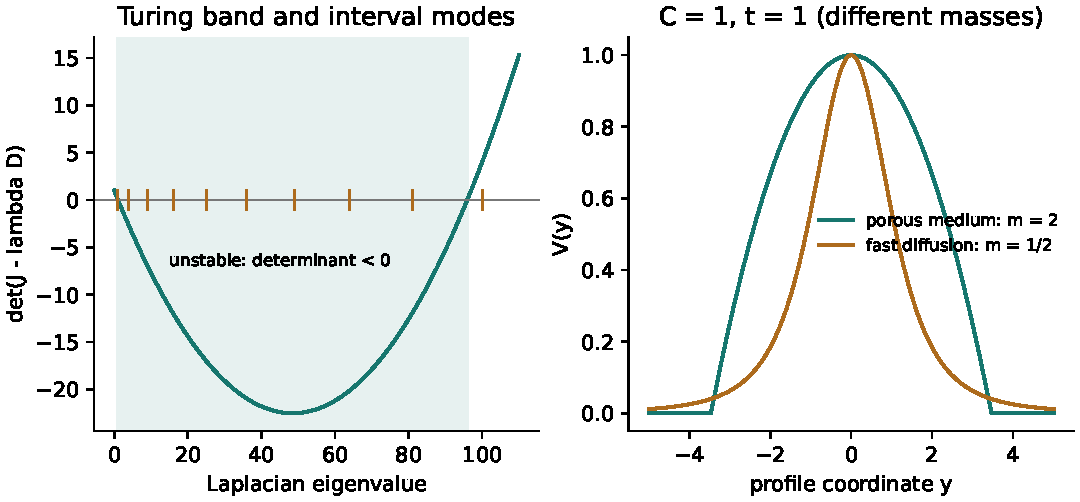
\includegraphics[width=\linewidth]{output/figures/ch04-modes-profiles.pdf}
\end{center}
\noindent\emph{Editorial figure.} The determinant band is compared with
the actual interval spectrum; the other panel compares scaling profiles.
\end{minipage}
% Evans second edition, section 4.2.
% English source: printed p. 167; PDF page 184 (1-based).
% Chinese subsection/page correspondence: pending verification against the scan.
% Status: outline-only; no source text or proof has been transcribed/reviewed.
\section{Similarity Solutions}
\label{sec:4-2}

\PDEPending

% TODO: English exposition with source theorem/equation identifiers.
% TODO: Add necessary \PDEVocab, \PDEIdea, or \PDEChinese notes.
% TODO: Expand abbreviated arguments in expandedproof/proofdetails.
% TODO: Verify hypotheses, endpoints, constants, limits, and cross-references.

% Evans 4.3.1, printed pp. 177--186; PDF pp. 194--203.
\Needspace{65mm}
\section{Transform Methods}\label{sec:4-3}
\Needspace{35mm}
\subsection{Fourier transform: normalization and Plancherel}
For $f\in L^1(\R^n)$ define
\[
 \begin{aligned}
 \widehat f(\xi)&=(2\pi)^{-n/2}\int e^{-ix\cdot\xi}f(x)\,dx,\\
 \mathcal F^{-1}h(x)&=(2\pi)^{-n/2}\int e^{ix\cdot\xi}h(\xi)\,d\xi .
 \end{aligned}
\]
The integrals are absolutely convergent.
For Schwartz functions integration by parts and Fubini yield
\[
 \widehat{\partial_j f}=i\xi_j\widehat f,\qquad
 \widehat{f*h}=(2\pi)^{n/2}\widehat f\,\widehat h .
 \tag{F4}
\]
For the second identity, set $x=z+y$ in the double integral.
Both normalizations must be retained; $\mathcal F$ is unitary,
whereas ordinary convolution has no normalizing factor.
\Needspace{45mm}
\PDEAnnotation{卷积公式为何多一个常数}{每个 Fourier 变换自带 $(2\pi)^{-n/2}$，两个变换相乘就出现两份。卷积只做一次变换，所以要乘回 $(2\pi)^{n/2}$；后面的核常数都由此决定。}


\PDEBodyDiagram{4.2}{Fourier transformation turns differentiation into multiplication.}
{The square commutes with the unitary normalization used here. There is no $2\pi$ in the multiplier because the exponential is $e^{-ix\cdot\xi}$. The heat multiplier is small at large $|\xi|$, connecting this representation with the stability picture in Chapter 1.}
{ch04-fourier-square}

\begin{theorem}[Plancherel and inversion; source Theorems 1--2]
The Fourier transform extends uniquely to a unitary operator on $L^2$.
It preserves inner products, has the displayed inverse, and
$\widehat{D^\gamma f}=(i\xi)^\gamma\widehat f$ whenever
the weak derivative is in $L^2$.
\end{theorem}
\begin{expandedproof}[Gaussian regularization without circular inversion]
\paragraph{1. The Gaussian transform.}
For $a>0$, $I(b)=\int_{\R} e^{-ax^2}e^{-ibx}\,dx$.
Differentiate under the integral and integrate by parts to get
$I'(b)=-bI(b)/(2a)$.
Since $I(0)=\sqrt{\pi/a}$,
$I(b)=\sqrt{\pi/a}\,e^{-b^2/(4a)}$.
Products give the $n$-dimensional identity.
This real-variable proof does not yet require contour deformation.

\paragraph{2. The norm identity.}
For $f\in L^1\cap L^2$ and $\eta>0$, Fubini gives
\[
 \int e^{-\eta|\xi|^2}|\widehat f(\xi)|^2\,d\xi
 =\iint f(x)\overline{f(y)}G_\eta(x-y)\,dx\,dy,
\]
where $G_\eta(z)=(4\pi\eta)^{-n/2}e^{-|z|^2/(4\eta)}$.
Fubini is legitimate since $\|f\|_1^2<\infty$ and the frequency
Gaussian is integrable.
The right side tends to $\|f\|_2^2$ because $G_\eta*f\to f$ in $L^2$.
For completeness,
\[
 \|G_\eta*f-f\|_2
 \leq\int G_\eta(z)\|f(\cdot-z)-f\|_2\,dz\longrightarrow0:
\]
translations are continuous in $L^2$ by approximation with compact
continuous functions; split the last integral into a small ball and
its Gaussian tail. Monotone convergence on the left gives the norm identity.
Polarization gives the inner-product identity.

\paragraph{3. Inversion and extension.}
For Schwartz $f$, (F4) implies rapid decay of $\widehat f$.
Fubini and the Gaussian formula give
\[
 \mathcal F^{-1}(e^{-\eta|\xi|^2}\widehat f)=G_\eta*f.
\]
The right side tends to $f$; the left tends to
$\mathcal F^{-1}\widehat f$ by dominated convergence.
Thus inversion holds on Schwartz functions.
Approximate arbitrary $L^2$ data by Schwartz functions.
The norm identity makes their transforms Cauchy and makes the limit
independent of the approximation. Inversion extends by continuity,
so the range is all of $L^2$.
Finally integration by parts against Schwartz tests proves the derivative
identity in distributions; if both sides belong to $L^2$, it is an
a.e. equality of those representatives.
\end{expandedproof}
\Needspace{45mm}
\PDEAnnotation{$L^2$ 变换不必是逐点积分}{一般 $L^2$ 函数未必可积，其 Fourier 变换通过范数极限定义。反演和乘子公式首先是 $L^2$ 等式；若要逐点表示，还须增加可积性或正则性。}

\Needspace{35mm}
\subsection{Fourier multipliers and evolution equations}
\paragraph{Bessel potential.}
For $-\Delta u+u=f$, $f\in L^2$,
$\widehat u=(1+|\xi|^2)^{-1}\widehat f$.
This gives a unique $L^2$ distributional solution with
$\int(1+|\xi|^2)^2|\widehat u|^2<\infty$.
A rigorous kernel representation is
\[
 K(x)=\int_0^\infty e^{-s}G_s(x)\,ds,\qquad u=K*f .
\]
Tonelli gives $K\geq0$ and $\|K\|_1=1$;
its transform is $(2\pi)^{-n/2}/(1+|\xi|^2)$.
The kernel called $B$ in the source is $(2\pi)^{n/2}K$.
The singularity of $K$ at zero in some dimensions does not prevent
its $L^1$ integrability or convolution action on $L^2$.
\Needspace{45mm}
\PDEAnnotation{乘子有界不表示核处处有限}{$(1+|\xi|^2)^{-1}$ 给出有界的 $L^2$ 乘子。对应核可能在原点无界，但仍可积；不能把一个点的奇性误当作表示公式失效。}

\paragraph{Heat and Schr\"odinger equations.}
Spatial transformation of $u_t-\Delta u=0$ gives
$\widehat u_t+|\xi|^2\widehat u=0$, hence
$\widehat u=e^{-t|\xi|^2}\widehat g$.
Gaussian inversion recovers $u=G_t*g$ from Chapter~2.
For $iu_t+\Delta u=0$ the sign is instead
$\widehat u_t=-i|\xi|^2\widehat u$, so
\[
 \widehat u=e^{-it|\xi|^2}\widehat g,\qquad
 u(x,t)=(4\pi it)^{-n/2}\int e^{i|x-y|^2/(4t)}g(y)\,dy .
 \tag{SC4}
\]
For $t\ne0$ use
$(it)^{-n/2}=|t|^{-n/2}e^{-i\pi n\,\operatorname{sgn}(t)/4}$.
The kernel identity follows by first replacing $it$ with $\eta+it$,
$\eta>0$, and then letting $\eta\downarrow0$.
For $g\in L^1\cap L^2$, the kernels converge under the spatial integral
by domination, while the multipliers converge in $L^2$.
Thus both descriptions agree.
For $L^2$ data this defines a unitary group:
\[
 \|u(t)\|_2=\|g\|_2,\qquad
 \|u(t)-g\|_2^2
 =\int|e^{-it|\xi|^2}-1|^2|\widehat g|^2\longrightarrow0 .
\]
If $g,|x|^2g\in L^1$, differentiation of (SC4) on compact
space-time sets away from $t=0$ verifies the classical PDE.
For arbitrary $L^2$ data the statement is distributional.
\Needspace{45mm}
\PDEAnnotation{色散与耗散的范数表现不同}{热乘子模长小于一，会压低高频；Schr\"odinger 乘子模长为一，保持 $L^2$。后者的点态衰减来自振荡抵消，不来自 $L^2$ 质量损失。}

\paragraph{Wave and telegraph equations.}
For $u_{tt}-\Delta u=0$, $u(0)=g$, $u_t(0)=h$,
\[
 \widehat u(\xi,t)=\cos(t|\xi|)\widehat g
              +\frac{\sin(t|\xi|)}{|\xi|}\widehat h.
 \tag{WV4}
\]
At $\xi=0$ the quotient is defined as $t$.
It is bounded by $t$, so the formula has no genuine zero-frequency pole.
For $u_{tt}+2du_t-u_{xx}=0$ use $\widehat u=e^{-dt}v$.
Then $v''+(\xi^2-d^2)v=0$ and
\[
 \widehat u=e^{-dt}
 \begin{cases}
 \cosh(qt)\widehat g+\dfrac{\sinh(qt)}q(\widehat h+d\widehat g),
                 &|\xi|<d,\ q=\sqrt{d^2-\xi^2},\\
 \widehat g+t(\widehat h+d\widehat g),&|\xi|=d,\\
 \cos(qt)\widehat g+\dfrac{\sin(qt)}q(\widehat h+d\widehat g),
                 &|\xi|>d,\ q=\sqrt{\xi^2-d^2}.
 \end{cases}
\]
These are the overdamped, critical and oscillatory regimes.
The common limiting formula at $q=0$ is essential.

\begin{theorem}[Asymptotic energy equipartition; source \S4.3.1]
If $g\in H^1(\R^n)$ and $h\in L^2(\R^n)$, the wave solution has
\[
 \|Du(t)\|_2^2\longrightarrow E_0,\qquad
 \|u_t(t)\|_2^2\longrightarrow E_0,\qquad
 E_0=\tfrac12(\|Dg\|_2^2+\|h\|_2^2).
\]
\end{theorem}
\begin{expandedproof}
Write $A=|\xi|\widehat g$ and $B=\widehat h$ in $L^2$.
Plancherel and (WV4) give
\[
 \|Du\|_2^2
 =\int|A|^2\cos^2(t|\xi|)+|B|^2\sin^2(t|\xi|)
       +2\operatorname{Re}(A\overline B)\sin(t|\xi|)\cos(t|\xi|).
\]
All three coefficient functions are $L^1$, the cross term by
Cauchy--Schwarz.
For any $F\in L^1(\R^n)$, polar coordinates give
$\int e^{2it|\xi|}F(\xi)\,d\xi=\int_0^\infty e^{2itr}H(r)\,dr$
with $\|H\|_1\leq\|F\|_1$.
The latter tends to zero: approximate $H$ in $L^1$ by smooth functions
supported inside $(0,\infty)$ and integrate those by parts.
Now use the double-angle identities to obtain the first limit.
The analogous formula for $u_t$ gives energy conservation and
the second limit.
This also handles $n=1$ without discarding a possible endpoint term
in a radial integration by parts.
\end{expandedproof}
% Supplement to Evans 4.3: Radon and Laplace transforms, printed pp. 186--195.
\Needspace{35mm}
\subsection{Radon transform and plane-wave decomposition}\label{sec:4-radon}
For $f\in C_c^\infty(\R^n)$, set
\[
 Rf(s,\omega)=\int_{x\cdot\omega=s}f(x)\,dS_x,\qquad \omega\in S^{n-1}.
\]
Coordinates $x=s\omega+\sum y_jb_j$, where $b_j$ are an orthonormal
basis of $\omega^\perp$, make the surface measure $dy$.
They immediately give
\[
 Rf(-s,-\omega)=Rf(s,\omega),\quad
 R(\partial_jf)=\omega_j\partial_sRf,\quad R(\Delta f)=\partial_s^2Rf .
\]
For the middle identity decompose $\partial_j$ into a normal and
tangential derivative. Tangential integrals vanish by compact support.
Induction gives $R(D^\gamma f)=\omega^\gamma\partial_s^{|\gamma|}Rf$.
If $\operatorname{supp}f\subset B_R$, then $Rf=0$ for $|s|\geq R$.


\PDEBodyDiagram{4.3}{Radon data integrate along level hyperplanes.}
{In dimension two the integration sets are lines perpendicular to $\omega$. The scalar $s$ is signed distance in the normal direction, not distance traveled along a line. The blue line is one member of the family; higher dimensions replace it by an $(n-1)$-plane.}
{ch04-radon-lines}

\begin{theorem}[Slice theorem and inversion; source Theorems 4--5]
With the unnormalized one-dimensional transform
$B(r,\omega)=\int_{\R} e^{-irs}Rf(s,\omega)\,ds$,
\[
 B(r,\omega)=(2\pi)^{n/2}\widehat f(r\omega).
\]
For every dimension,
\[
 f(x)=\frac1{2(2\pi)^n}
 \int_{S^{n-1}}\int_{\R} B(r,\omega)|r|^{n-1}e^{irx\cdot\omega}\,dr\,dS_\omega .
\]
If $n=2k+1$ is odd, this becomes the local formula
\[
 f(x)=C_n\int_{S^{n-1}}
       \partial_s^{2k}Rf(x\cdot\omega,\omega)\,dS_\omega,\qquad
 C_n=\frac{(-1)^k}{2(2\pi)^{2k}} .
 \tag{RI4}
\]
\end{theorem}
\begin{expandedproof}
Fubini in the orthonormal coordinates gives
\[
 B(r,\omega)=\int f(x)e^{-ir\omega\cdot x}\,dx .
\]
In Fourier inversion, polar coordinates with signed $r$ double-count
each nonzero frequency, giving the factor $1/2$ and $|r|^{n-1}$.
All integrals converge since $\widehat f$ is rapidly decreasing.
For $n-1=2k$, one-dimensional inversion gives
\[
 \partial_s^{2k}Rf(s,\omega)
 =\frac{(-1)^k}{2\pi}\int_{\R} r^{2k}B(r,\omega)e^{irs}\,dr .
\]
Substituting this in the general inversion formula proves (RI4).
\end{expandedproof}
\Needspace{45mm}
\PDEAnnotation{奇偶维差别藏在绝对值里}{带符号的极径在一般维数必须用 $|r|^{n-1}$；只有奇维时才等于多项式 $r^{2k}$，从而变成有限阶局部导数。偶维的反演通常带非局部算子。}

For odd $n$, define $\rho_f=C_n\partial_s^{n-1}Rf$.
Then the plane-wave integral
\[
 u(x,t)=\int_{S^{n-1}}\rho_g(x\cdot\omega-t,\omega)\,dS_\omega
\]
solves $u_{tt}-\Delta u=0$, $u(0)=g$, $u_t(0)=0$.
The PDE holds because $|\omega|=1$; the first initial condition is
(RI4). The integrand for $u_t(0)$ is odd under $\omega\mapsto-\omega$,
since an odd $s$ derivative reverses the symmetry of $Rg$.

For the constant-coefficient system
$\mathbf u_t+\sum B_j\mathbf u_{x_j}=0$,
suppose $B(\omega)=\sum\omega_jB_j$ is diagonalizable with real
eigenvalues $\lambda_l(\omega)$.
In Radon coordinates the diagonal components satisfy one-dimensional
transport and equal
\[
 v_l(s,\omega,t)=h_l(s-\lambda_l(\omega)t,\omega).
\]
After applying (RI4), use
$\rho_l(s,\omega)=C_n\partial_s^{n-1}h_l(s,\omega)$ exactly once:
\[
 \mathbf u(x,t)=\int_{S^{n-1}}\sum_l
 a_l(\omega)\rho_l(x\cdot\omega-\lambda_l(\omega)t,\omega)\,dS_\omega .
\]
Here $a_l$ are the diagonalizing columns; the shift is not inserted
again in the definition of $\rho_l$.
For compact data in $B_R$, if
$\min_{\omega,l}|\lambda_l(\omega)|=\sigma>0$,
then $\mathbf u=0$ for $|x|<\sigma t-R$.
Indeed each shifted argument has magnitude at least $\sigma t-|x|>R$.
This is a conditional odd-dimensional Huygens statement; the
diagonalization and nonzero-speed hypotheses cannot be removed.
\Needspace{45mm}
\PDEAnnotation{平面支集条件怎样变成内部空区}{若 $|x|<\sigma t-R$，所有方向的平面参数都移出初始支集区间，整个反演积分为零。零特征速度会留下不移动的分量，因此必须单独排除。}

\Needspace{35mm}
\subsection{Laplace transform, resolvents and the heat--wave link}
If $v$ and $v_t$ have suitable exponential bounds, integration by parts gives
\[
 \mathcal L(v_t)(s)=s\mathcal Lv(s)-v(0),\qquad
 \mathcal Lv(s)=\int_0^\infty e^{-st}v(t)\,dt .
\]
Thus for $v_t-\Delta v=0$, $v(0)=f$,
\[
 (s-\Delta)\mathcal Lv=f .
\]
Use the same spatial boundary condition before and after transformation;
for example a zero Dirichlet condition stays zero.
In the whole space this recovers
$(s-\Delta)^{-1}f=\int_0^\infty e^{-st}(G_t*f)\,dt$.
For $L^2$ data the Bochner integral is justified by
$\|G_t*f\|_2\leq\|f\|_2$.
\Needspace{45mm}
\PDEAnnotation{初值正是 Laplace 分部积分的边界项}{时间导数并非只替换成乘以 $s$。零时刻留下 $-v(0)$，它成为椭圆 resolvent 方程的右端；漏掉这一项就把非零初值问题变成了齐次问题。}

\begin{theorem}[Gaussian averaging of the wave group; source Example 9]
Let $g$ be smooth compactly supported, and let $U(x,s)$ be the wave
solution with displacement $g$ and zero initial velocity, extended evenly
in $s$. Then
\[
 V(x,t)=\frac1{\sqrt{4\pi t}}\int_{\R} e^{-s^2/(4t)}U(x,s)\,ds
\]
is the heat solution with datum $g$.
\end{theorem}
\begin{expandedproof}
For smooth data the derivatives of $U$ grow at most polynomially,
as can also be checked from its Fourier representation.
Gaussian weights justify differentiation and kill the boundary terms.
Writing $q_t(s)=(4\pi t)^{-1/2}e^{-s^2/(4t)}$, observe
$\partial_tq_t=\partial_{ss}q_t$. Hence
\[
 V_t=\int q_{ss}U=\int qU_{ss}=\int q\Delta U=\Delta V.
\]
The Gaussian approximate identity in $s$ gives $V(0)=g$.
Alternatively the frequency multiplier is
$\int q_t(s)\cos(s|\xi|)\,ds=e^{-t|\xi|^2}$,
which proves the same statement in $L^2$.
\end{expandedproof}

For $n=2k+1\geq3$, let $M_g(x,r)$ be the spherical average of $g$.
Equating the two Gaussian representations gives, with
$\lambda=1/(4t)$,
\[
 \int_0^\infty e^{-\lambda s^2}U(x,s)\,ds
 =\frac{|S^{n-1}|}{2\pi^k}\lambda^k
       \int_0^\infty e^{-\lambda r^2}r^{2k}M_g(x,r)\,dr .
\]
Use $\lambda e^{-\lambda r^2}=-(2r)^{-1}\partial_re^{-\lambda r^2}$
and integrate by parts $k$ times. The result is
\[
 \lambda^k\int_0^\infty e^{-\lambda r^2}r^{2k}M_g\,dr
 =2^{-k}\int_0^\infty e^{-\lambda r^2}
       r(r^{-1}\partial_r)^k(r^{2k-1}M_g)\,dr .
\]
There are no boundary terms at infinity by compact support in $r$.
At zero, $M_g$ is smooth and even; before the last differentiation
the relevant odd power has not fallen below one, so the boundary
terms are zero.
After $s^2=\tau$, uniqueness of the Laplace transform implies
\[
 U(x,t)=\frac1{(n-2)!!}\,
 \partial_t(t^{-1}\partial_t)^{(n-3)/2}
                  (t^{n-2}M_g(x,t)).
\]
Here $|S^{n-1}|/(2^{k+1}\pi^k)=1/(n-2)!!$ follows from the
Gaussian sphere area formula.
The one-dimensional case is $U=(g(x+t)+g(x-t))/2$.
One can justify Laplace uniqueness without a new PDE theorem:
after multiplying by $e^{-a\tau}$, substitute $z=e^{-\tau}$;
vanishing at all $s=a+j$ gives zero moments on $[0,1]$.
Polynomial density in continuous functions makes the finite signed
measure zero. This applies to the continuous, exponentially integrable
functions above.


% Evans second edition, section 4.4.
% English source: printed p. 195; PDF page 212 (1-based).
% Chinese subsection/page correspondence: pending verification against the scan.
% Status: outline-only; no source text or proof has been transcribed/reviewed.
\section{Converting Nonlinear into Linear PDE}
\label{sec:4-4}

\PDEPending

% TODO: English exposition with source theorem/equation identifiers.
% TODO: Add necessary \PDEVocab, \PDEIdea, or \PDEChinese notes.
% TODO: Expand abbreviated arguments in expandedproof/proofdetails.
% TODO: Verify hypotheses, endpoints, constants, limits, and cross-references.

% Evans 4.5.1--2, printed pp. 200--206; PDF pp. 217--223.
\Needspace{65mm}
\section{Asymptotics}\label{sec:4-5}
The source presents several asymptotic constructions formally.
We distinguish exact algebraic identities, proved local integral
asymptotics, and conditional PDE expansions.
No convergence theorem is inferred merely by matching powers.

\Needspace{35mm}
\subsection{A small-diffusion plume: geometry and transverse scale}
Consider $\operatorname{div}(\mathbf b\,\mu)=\delta_0$ in two dimensions.
Let $\dot X=\mathbf b(X)$, $X(0)=0$, and suppose $|\mathbf b(X)|>0$.
If the forward trajectory leaves compact sets, the locally finite measure
\[
 \int\phi\,d\mu=\int_0^\infty\phi(X(t))\,dt
\]
solves this equation, since
\[
 -\int\mathbf b\cdot D\phi\,d\mu
 =-\int_0^\infty\frac d{dt}\phi(X(t))\,dt=\phi(0).
\]
This is an outgoing solution; an extra background homogeneous solution
is not excluded by this calculation.
With speed $\sigma=|\mathbf b(X)|$, tangent $\tau$ and unit normal $\nu$,
use $x=X(t)+y\nu(t)$ in a nonoverlapping tubular neighborhood.
Frenet identities give $\nu'=-\sigma\kappa\tau$ and
\[
 x_t=\sigma(1-\kappa y)\tau,\quad x_y=\nu,\quad
 dx=H\,dt\,dy,\qquad H=\sigma(1-\kappa y)>0.
\]
Thus the same measure has density $\delta(y)/\sigma(t)$ with respect
to spatial area.
\Needspace{45mm}
\PDEAnnotation{线上的密度必须带速度因子}{注入量按行进时间计量，而面积元在曲线处含 $\sigma(t)$。因此横向 Dirac 前要乘 $1/\sigma$。若轨道封闭或反复回返，时间积分可能不是局部有限测度。}

Now perturb to $-\varepsilon\Delta u^\varepsilon+
\operatorname{div}(\mathbf b u^\varepsilon)=\delta_0$.
Away from the injection point, set
$z=y/\sqrt\varepsilon$,
$u^\varepsilon=\varepsilon^{-1/2}v^\varepsilon(t,z)$.
The coordinate metric gives the exact identity
\[
 \Delta w=\frac1H\partial_t(H^{-1}w_t)
                  +\frac1H\partial_y(Hw_y).
\]
Also write
$\mathbf b=(\sigma+\alpha y+O(y^2))\tau+
(\beta y+O(y^2))\nu$.
Then on compact $t>0$, bounded $z$, provided the needed derivatives
of $v^\varepsilon$ are uniformly bounded,
\[
 \mathbf b\cdot Dv^\varepsilon
       =v^\varepsilon_t+\beta z v^\varepsilon_z+O(\sqrt\varepsilon),
 \qquad
 \varepsilon\Delta v^\varepsilon=v^\varepsilon_{zz}+O(\sqrt\varepsilon),
\]
\[
 \operatorname{div}\mathbf b
       =\sigma'/\sigma+\beta+O(\sqrt\varepsilon).
\]
For example the transverse first-derivative term in the Laplacian
is $\varepsilon(H_y/H)\partial_yv^\varepsilon=O(\sqrt\varepsilon)$;
the tangential second-derivative terms are $O(\varepsilon)$.
Thus the conditional leading equation is
\[
 v_t-v_{zz}+(\beta z v)_z+(\sigma'/\sigma)v=0,\qquad
 v(0)=\delta_0/\sigma(0).
 \tag{PL4}
\]
Its exact Gaussian solution, derived again in Problem 13, is
\[
 v(t,z)=\frac{e^{-z^2/\Gamma(t)}}{\sigma(t)\sqrt{\pi\Gamma(t)}},
 \qquad \Gamma'=4+2\beta\Gamma,\quad\Gamma(0)=0 .
\]
Indeed $A=\sigma v$ satisfies $A_t=A_{zz}-(\beta zA)_z$;
substituting the Gaussian gives the displayed ODE and mass $\int A=1$.
The transverse width is $\sqrt{\varepsilon\Gamma(t)}$.
This does not by itself prove approximation of the original elliptic
Green function, nor control the injection region or large times.
\Needspace{45mm}
\PDEAnnotation{形式余项依赖尚未证明的统一界}{把 $y$ 换成 $\sqrt\varepsilon z$ 后，系数误差很小，但它仍乘着解的导数。只有这些导数在所考察区域有统一界，才能写成统一的 $O(\sqrt\varepsilon)$。}

\Needspace{35mm}
\subsection{Laplace concentration and vanishing viscosity}\label{sec:4-laplace}
\begin{lemma}[Source asymptotics lemma, with tail control]
Let $k,l$ be continuous on $\R$, $|l(y)|\leq C(1+|y|)$,
and $k(y)\geq c y^2-C$, $c>0$.
If $k$ has a unique minimum at $y_0$, then
\[
 \frac{\int l(y)e^{-k(y)/\varepsilon}\,dy}
      {\int e^{-k(y)/\varepsilon}\,dy}\longrightarrow l(y_0).
 \tag{LC4}
\]
\end{lemma}
\begin{expandedproof}
Subtract the minimum $k_0$ and put $h=k-k_0\geq0$.
Fix a small neighborhood $N$ of $y_0$ on which
$|l-l(y_0)|<\eta$.
On a large compact interval outside $N$, $h\geq d>0$ by uniqueness.
Increase the interval so that outside it
$h(y)\geq d/2+(c/2)y^2$, decreasing $d$ if necessary.
By continuity there is an interval of length $2r>0$ near $y_0$
where $h<d/4$.
The denominator is at least $2r e^{-d/(4\varepsilon)}$.
The numerator of the absolute error over the compact complement
is at most $C_1e^{-d/\varepsilon}$.
The tail numerator is bounded by
\[
 C_2e^{-d/(2\varepsilon)}
       \int(1+|y|)e^{-cy^2/(2\varepsilon)}\,dy,
\]
whose ratio to the denominator tends to zero.
Inside $N$ the normalized error is at most $\eta$.
Let $\varepsilon\downarrow0$ and then $\eta\downarrow0$.
This proves concentration together with the required control of
the unbounded observable $l$.
\end{expandedproof}
\Needspace{45mm}
\PDEAnnotation{逐点密度趋零不足以推出集中}{归一化密度在每个非极小点趋零，还不能控制积分或无穷远的质量。证明需要分母下界、远离极小点的能量间隙，以及带权尾积分。}

For bounded initial $g$, let $P'=g$ and
$K(y)=(x-y)^2/(2t)+P(y)$.
The quadratic term dominates the Lipschitz primitive.
Formula (VB4) and (LC4), with parameter $2\varepsilon$, imply
\[
 u^\varepsilon(x,t)\longrightarrow \frac{x-y(x,t)}t
\]
whenever the minimizing point is unique.
By Chapter~3, at each $t>0$ only countably many $x$ have multiple
minimizers, and the right side is the Lax--Oleinik entropy solution.
Since $|u^\varepsilon|\leq\|g\|_\infty$, this convergence is also
$L^1_{\rm loc}$ in $x$ for each fixed $t$.
Joint a.e. convergence and the same bound give local space-time
$L^1$ convergence away from zero.
The multiple-minimizer set is measurable, for instance by expressing
separation of two minimizers using rational compact neighborhoods;
Fubini therefore applies to the countable time slices.
\Needspace{45mm}
\PDEAnnotation{与第三章的最小化公式接上了}{黏性解是最优速度的指数加权平均。黏性趋零时，权重集中到作用量最低点；最低点的分支竞争正对应守恒律的激波。}

If $k$ is smooth with finitely many nondegenerate global minima $y_j$,
local Taylor expansion $y=y_j+\sqrt\varepsilon z$ and Gaussian
domination give
\[
 \int l e^{-k/\varepsilon}
 =e^{-k_0/\varepsilon}\sqrt{2\pi\varepsilon}
       \left(\sum_j\frac{l(y_j)}{\sqrt{k''(y_j)}}+o(1)\right).
\]
To justify domination, restrict to a small neighborhood where
$k-k_0\geq c_j|y-y_j|^2$, and use the energy gap outside.
Thus at a tie the limit is a weighted average, not necessarily
the velocity at one selected minimizing point.
Values on shock curves do not affect the weak solution.
% Supplement to Evans 4.5.3, printed pp. 207--217.
\Needspace{35mm}
\subsection{Geometric optics and stationary phase}\label{sec:4-stationary}
For $u^\varepsilon=a e^{ip/\varepsilon}$ the exact wave-operator identity is
\[
 \begin{aligned}
 &e^{-ip/\varepsilon}(u^\varepsilon_{tt}-\Delta u^\varepsilon)\\
 &\quad=\varepsilon^{-2}a(|Dp|^2-p_t^2)\\
 &\qquad+\frac{i}{\varepsilon}
       \{2p_ta_t-2Dp\cdot Da+a(p_{tt}-\Delta p)\}
       +(a_{tt}-\Delta a).
 \end{aligned}
\]
Matching the first two orders gives the eikonal and amplitude equations
\[
 p_t^2=|Dp|^2,\qquad
 2p_ta_t-2Dp\cdot Da+(p_{tt}-\Delta p)a=0 .
\]
On a smooth nonzero-frequency branch choose $p_t=\pm|Dp|$.
The sign cannot be chosen independently at every point.
For $u_{tt}-\sum a_{ij}(x)u_{x_ix_j}=0$ the first equation becomes
$p_t^2=\sum a_{ij}p_{x_i}p_{x_j}$, with the corresponding amplitude
expression obtained by the same differentiation.
These identities define a candidate expansion.
A theorem about exact solutions needs control of the residual and
the evolution, especially near caustics.
\Needspace{45mm}
\PDEAnnotation{相位误差除以小参数会放大}{即使 $p^\varepsilon-p=o(1)$，也不能直接推出两个指数相近；指数里的差是 $(p^\varepsilon-p)/\varepsilon$。振荡展开需要比普通逐点收敛更精确的误差尺度。}

\begin{lemma}[Nonstationary phase; strengthening source Lemma 1]
If $a\in C_c^\infty$ and $|D\phi|>0$ on its support, then for every
integer $N\geq1$,
$\int e^{i\phi/\varepsilon}a=O(\varepsilon^N)$.
\end{lemma}
\begin{expandedproof}
Near the support let $V=D\phi/|D\phi|^2$.
Then $V\cdot D e^{i\phi/\varepsilon}=(i/\varepsilon)e^{i\phi/\varepsilon}$.
Integration by parts gives
\[
 \int e^{i\phi/\varepsilon}a
 =-\frac{\varepsilon}{i}\int e^{i\phi/\varepsilon}
                                  \operatorname{div}(aV).
\]
Iterate $N$ times; the final smooth compactly supported amplitude
has finite $L^1$ norm independent of $\varepsilon$.
This also proves the source's linear-phase case.
\end{expandedproof}

\begin{lemma}[Quadratic phase; source Lemma 2]
For real symmetric invertible $H$ and $a\in C_c^\infty(\R^d)$,
\[
 \int e^{iz\cdot Hz/(2\varepsilon)}a(z)\,dz
 =(2\pi\varepsilon)^{d/2}
   \frac{e^{i\pi\operatorname{sgn}H/4}}{|\det H|^{1/2}}
      [a(0)+O(\varepsilon)].
 \tag{QP4}
\]
\end{lemma}
\begin{expandedproof}[regularization, branch and error]
For $\operatorname{Re}q>0$,
\[
 \int_{\R} e^{-qs^2+ibs}\,ds=\sqrt{\pi}\,q^{-1/2}e^{-b^2/(4q)} .
\]
Choose the square root with positive real part.
For real positive $q$ this is the Gaussian identity; analytic
continuation in the right half-plane proves it for complex $q$,
since compact subsets admit an integrable Gaussian majorant.
Equivalently the contour argument of Problem 15 proves it directly.

Diagonalize $H$ orthogonally, multiply the phase by
$e^{-\eta|z|^2}$, and apply this identity in each coordinate.
As $\eta\downarrow0$, an eigenvalue $\lambda$ contributes the factor
$|\lambda|^{-1/2}e^{i\pi\operatorname{sgn}\lambda/4}$ after the common
$(2\pi\varepsilon)^{1/2}$ factor.
Insert Fourier inversion for $a$ before this calculation.
Its transform is rapidly decreasing.
The regularized Gaussian integral is uniformly bounded in frequency,
so dominated convergence yields the exact oscillatory identity
\[
 \begin{aligned}
 \int e^{iz\cdot Hz/(2\varepsilon)}a(z)\,dz
 &=C_{\varepsilon,H}(2\pi)^{-d/2}\\
 &\quad\cdot\int \widehat a(\xi)
                e^{-i\varepsilon\xi\cdot H^{-1}\xi/2}\,d\xi ,
 \end{aligned}
\]
where $C_{\varepsilon,H}$ is the prefactor in (QP4).
Since $|e^{ir}-1|\leq|r|$, the bracket differs from $a(0)$ by at most
\[
 C\varepsilon\int |\xi|^2|\widehat a(\xi)|\,d\xi<\infty .
\]
This proves both the constant and the error in (QP4).
\end{expandedproof}

\begin{lemma}[Morse coordinates; source Lemma 3(ii)]
If $D\phi(0)=0$ and $H=D^2\phi(0)$ is invertible, there is a local
smooth diffeomorphism $\Phi$ with $\Phi(0)=0$, $D\Phi(0)=I$, and
$\phi(\Phi(z))=\phi(0)+z\cdot Hz/2$.
\end{lemma}
\begin{expandedproof}[an editorial matrix proof]
Taylor's formula with integral remainder gives
$\phi(x)=\phi(0)+x^TA(x)x/2$, where
$A(x)=2\int_0^1(1-s)D^2\phi(sx)\,ds$ and $A(0)=H$.
On symmetric matrices solve
\[
 H+2S+SH^{-1}S=A(x).
\]
The derivative in $S$ at zero is $2I$, so the implicit function
theorem gives a smooth symmetric $S(x)$ with $S(0)=0$.
Set $B=I+H^{-1}S$; then $B^THB=A$.
The map $z=B(x)x$ has derivative $I$ at zero.
Its local inverse $\Phi$ has the required properties.
This works for indefinite $H$ as well as positive definite $H$.
\end{expandedproof}
For completeness the source's noncritical coordinate lemma is also
elementary. Choose rows $r_1,\ldots,r_{d-1}$ complementary to
$D\phi(0)$, impose $r_j\cdot(y-x)=0$ and
$\phi(y)-\phi(0)=D\phi(0)\cdot x$.
The $y$ Jacobian is invertible; the implicit function theorem
gives $y=\Phi(x)$ and differentiation gives $D\Phi(0)=I$.


\PDEBodyDiagram{4.4}{Near a nondegenerate stationary point the scale is square-root.}
{For phase $x^2$, oscillation is slow near its stationary point at zero and rapid farther away. The highlighted interval has width $2\sqrt{\varepsilon}$. Rescaling $x=\sqrt{\varepsilon}\,z$ explains the leading $\varepsilon^{1/2}$ factor in one dimension; cancellation, not pointwise smallness of the integrand, suppresses the outer region.}
{ch04-stationary-window}

\begin{theorem}[Nondegenerate stationary phase]
Suppose $\phi$ has just finitely many critical points $z_j$ on
$\operatorname{supp}a$, and all $H_j=D^2\phi(z_j)$ are invertible.
Then
\[
 \int e^{i\phi(z)/\varepsilon}a(z)\,dz
 =(2\pi\varepsilon)^{d/2}
 \sum_j\frac{e^{i\phi(z_j)/\varepsilon+i\pi\operatorname{sgn}H_j/4}}
                 {|\det H_j|^{1/2}}
                  [a(z_j)+O(\varepsilon)].
 \tag{SP4}
\]
\end{theorem}
\begin{expandedproof}
Choose a partition of unity separating small neighborhoods of the
critical points from the noncritical compact remainder.
The latter is $O(\varepsilon^N)$ for arbitrary $N$ by the first lemma.
At each critical point change to Morse coordinates.
The transformed amplitude is $a(\Phi(z))|\det D\Phi(z)|$
times its cutoff and equals $a(z_j)$ at the origin.
Apply (QP4) to each localized integral and add them.
Taking $N>d/2+1$ absorbs the noncritical remainder.
\end{expandedproof}
\Needspace{45mm}
\PDEAnnotation{行列式为零时不能继续用驻相公式}{$|\det H|^{-1/2}$ 描述非退化临界点的集中强度。它发散时，表示这一阶近似失效；需研究更高阶相位，不能把发散系数直接当作精确解的无穷大。}

\paragraph{Recovering the rays of Chapter 3.}
For high-frequency displacement $g^\varepsilon(z)=a(z)e^{ip_0(z)/\varepsilon}$
with $|Dp_0|>0$ on $\operatorname{supp}a$ and zero initial velocity,
Fourier representation splits the wave into two equal half-waves.
After frequency rescaling their phases are
\[
 \phi_\pm(x,y,z,t)=(x-z)\cdot y\pm t|y|+p_0(z).
\]
The critical equations are
\[
 y=Dp_0(z),\qquad x=z\mp t\,\frac{Dp_0(z)}{|Dp_0(z)|}.
 \tag{RAY4}
\]
These are exactly the projected HJ rays for $p_t\mp|Dp|=0$.
The joint Hessian at a critical point is
\[
 \begin{pmatrix}
 \displaystyle\pm\frac t{|y|}(I-\widehat y\otimes\widehat y)&-I\\
 -I&D^2p_0(z)
 \end{pmatrix},\qquad \widehat y=y/|y|.
\]
Its determinant equals $(-1)^n$ times the Jacobian determinant
of the ray map in (RAY4), by block elimination.
For small time that map is locally invertible.
The critical value is $p_0(z)$, since
$(x-z)\cdot y\pm t|y|=0$.
Applying (SP4) in $2n$ variables cancels the half-wave prefactor
$(2\pi\varepsilon)^{-n}$ and gives the amplitude
$a(z)/|\det D_zx|^{1/2}$ and the Hessian signature phase.
The two half-waves are then added with weight $1/2$.

The amplitude in $y,z$ is initially not compact in $y$.
To justify this application, first cut frequencies off to a compact
neighborhood of $Dp_0(\operatorname{supp}a)$ disjoint from zero.
Outside that neighborhood $D_z\phi=Dp_0-y$ is nonzero.
Repeated integration by parts in $z$ makes the tail integrable in
$y$, with arbitrarily high powers of $\varepsilon$; for large $y$
each integration also supplies inverse powers of $|y|$.
This reduces to the compactly supported theorem.
The formula is local before caustics or summed over the finitely many
nondegenerate preimages; it asserts no uniform approximation at a caustic.
\par\noindent\begin{minipage}{\linewidth}
\begin{center}
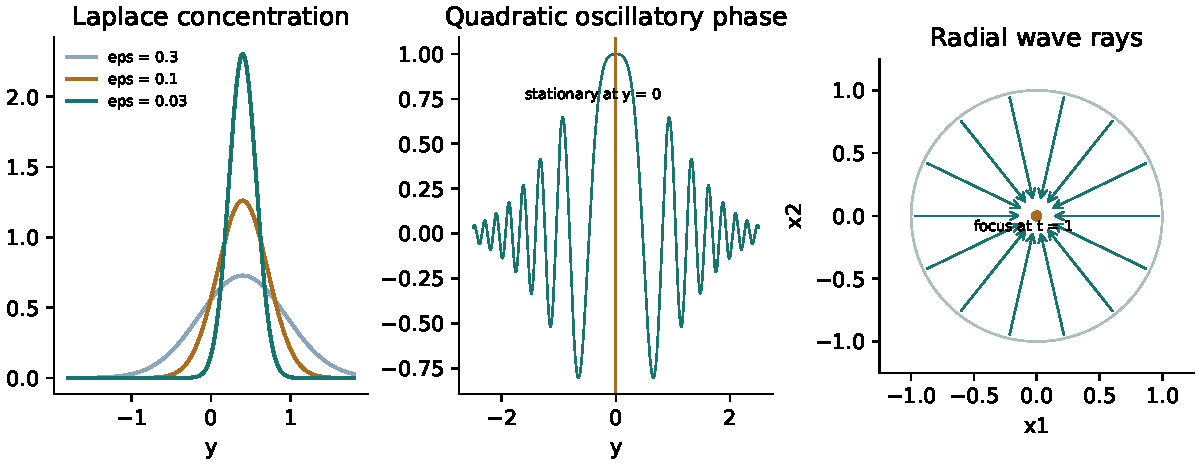
\includegraphics[width=\linewidth]{output/figures/ch04-concentration-rays.pdf}
\end{center}
\noindent\emph{Editorial figure.} Laplace concentration is compared
with oscillatory cancellation; the ray diagram displays a focusing map
whose Jacobian eventually vanishes.
\end{minipage}

% Supplement to Evans 4.5.4, printed pp. 217--220.
\Needspace{35mm}
\subsection{Periodic homogenization: expansion, cell problem, and a proof}
\label{sec:4-homogenization}
We use the symmetric uniformly elliptic case, sufficient also for
Problem 18: $A(y)=A(y)^T$ is smooth, $Q$-periodic,
$Q=(0,1)^n$, and $\theta I\leq A\leq\Theta I$.
Consider $-\operatorname{div}(A(x/\varepsilon)Du^\varepsilon)=f$
on a bounded Lipschitz domain with zero trace and $f\in L^2$.
The source uses a formal expansion; we first derive it, then give
a weak-convergence proof under these stated hypotheses.

\paragraph{Two-scale bookkeeping.}
Write $u^\varepsilon=u_0(x,y)+\varepsilon u_1(x,y)+\cdots$,
$y=x/\varepsilon$, with all $u_j$ periodic in $y$.
Every spatial derivative becomes $D_x+\varepsilon^{-1}D_y$.
Thus the three operator pieces are
\[
 L_1=-D_y\cdot AD_y,\quad
 L_2=-D_y\cdot AD_x-D_x\cdot AD_y,\quad
 L_3=-D_x\cdot AD_x .
\]
The coefficients of $\varepsilon^{-2},\varepsilon^{-1},1$ give
\[
 L_1u_0=0,\quad L_1u_1+L_2u_0=0,\quad
 L_1u_2+L_2u_1+L_3u_0=f .
\]
Testing the first identity by $u_0$ and integrating over $Q$ gives
$D_yu_0=0$; opposite periodic faces cancel.
For zero-mean correctors $\chi_i$, define
\[
 \operatorname{div}_y\{A(y)(e_i-D_y\chi_i)\}=0,\qquad
 \int_Q\chi_i=0 .
 \tag{CELL4}
\]
Then $u_1=-\sum_i\chi_i(y)u_{x_i}$ solves the next equation.
Averaging the order-one equation kills $L_1u_2$ and yields
\[
 -\operatorname{div}(\overline A Du)=f,\qquad
 \overline A e_i=\int_Q A(y)(e_i-D\chi_i)\,dy .
 \tag{HOM4}
\]
The minus sign in $u_1$ matches the source's corrector convention.
Many other texts use $\varphi_i=-\chi_i$ and a plus sign instead.

\Needspace{45mm}
\PDEAnnotation{平均的是修正后的通量}{有效系数通常不是直接对 $A$ 求平均。微观梯度要先调整成 $e_i-D\chi_i$，使通量在单元中无散，再取平均；一维时结果是调和平均而非算术平均。}

\PDEMarginDiagram{4.M}{一维有效系数}
{两个半格串联时通量相同，梯度与系数成反比。平均的是阻力 $1/a$，再取倒数。分段常系数可按弱形式理解。}
{ch04-cell-margin}

\begin{lemma}[Cell solvability and effective ellipticity]
(CELL4) has a unique zero-mean periodic weak solution.
The matrix $\overline A$ is symmetric and satisfies
$\theta I\leq\overline A\leq\Theta I$.
\end{lemma}
\begin{expandedproof}
On the zero-mean periodic $H^1$ space minimize
$\int_Q(e_i-Dv)\cdot A(e_i-Dv)$.
Periodic Poincar\'e and ellipticity bound every minimizing sequence
in $H^1$; weak compactness and weak lower semicontinuity give a minimizer.
The first variation is
$\int_Q A(D\chi_i-e_i)\cdot D\psi=0$.
Strict convexity in the gradient makes the difference of two
minimizers constant, hence zero after normalization.
These are standard Hilbert-space compactness and periodic Poincar\'e
facts; the cell equation is not solved merely by asserting zero mean.

For $\xi\in\R^n$, let $\chi_\xi=\sum_i\xi_i\chi_i$.
The cell identity allows any gradient $D\chi_\eta$ to be subtracted
from the other factor, so
\[
 \eta\cdot\overline A\xi
 =\int_Q(\eta-D\chi_\eta)\cdot A(\xi-D\chi_\xi).
\]
This proves symmetry.
The minimum over all periodic $v$ equals
$\xi\cdot\overline A\xi$ by orthogonality.
Its lower bound is
$\theta\int_Q|\xi-Dv|^2\geq\theta|\xi|^2$,
since $\int_QDv=0$ and $|Q|=1$.
The competitor $v=0$ gives the upper bound.
\end{expandedproof}

\begin{theorem}[An editorial rigorous homogenization statement]
Under the symmetric hypotheses above,
$u^\varepsilon\rightharpoonup u$ in $H_0^1$ and
$u^\varepsilon\to u$ in $L^2$, where $u$ is the unique weak solution of (HOM4).
\end{theorem}
\begin{expandedproof}[oscillating tests replace an unproved expansion]
Testing the original PDE by $u^\varepsilon$ gives a uniform $H_0^1$
bound by ellipticity and Poincar\'e.
Take a weakly convergent subsequence and use Rellich for strong $L^2$
convergence. The fluxes
$\eta^\varepsilon=A(x/\varepsilon)Du^\varepsilon$
are bounded in $L^2$; take a weak limit $\eta$.
The PDE gives $-\operatorname{div}\eta=f$.

For each $i$ put
\[
 w_i^\varepsilon=x_i-\varepsilon\chi_i(x/\varepsilon),\qquad
 q_i^\varepsilon=A(x/\varepsilon)Dw_i^\varepsilon .
\]
Periodic averaging implies $w_i^\varepsilon\to x_i$ in $L^2_{\rm loc}$
and $q_i^\varepsilon\rightharpoonup\overline A e_i$ in $L^2_{\rm loc}$;
also $\operatorname{div}q_i^\varepsilon=0$.
The averaging fact follows first by summing integrals on full
$\varepsilon$-cells for continuous periodic functions and compact tests,
then by $L^2(Q)$ approximation and uniform local cell bounds.

For $\phi\in C_c^\infty(U)$ symmetry gives
$\eta^\varepsilon\cdot Dw_i^\varepsilon
=Du^\varepsilon\cdot q_i^\varepsilon$.
Integrate the two sides by parts in different ways:
\[
 \int\phi\,\eta^\varepsilon\cdot Dw_i^\varepsilon
 =\int f\phi w_i^\varepsilon-\int w_i^\varepsilon\eta^\varepsilon\cdot D\phi,
\]
\[
 \int\phi\,Du^\varepsilon\cdot q_i^\varepsilon
 =-\int u^\varepsilon q_i^\varepsilon\cdot D\phi .
\]
Every product in these two right sides has a strong $L^2$ factor
and a weak $L^2$ factor.
The limits give $\eta_i=Du\cdot\overline A e_i$.
By symmetry this says $\eta=\overline A Du$, proving (HOM4).
Effective ellipticity gives uniqueness, so every subsequence has the
same limit; the entire family converges.
\end{expandedproof}
\Needspace{45mm}
\PDEAnnotation{两个弱收敛量不能直接相乘}{$A(x/\varepsilon)$ 与 $Du^\varepsilon$ 都会振荡，不能分别取弱极限再相乘。振荡测试把乘积改写为一个强收敛因子和一个弱收敛因子的配对，才识别出有效通量。}
The expansion need not satisfy the original boundary condition termwise;
boundary layers may be necessary for a quantitative error estimate.
We have proved weak $H^1$ convergence, not strong convergence of
the gradients or an $O(\varepsilon)$ global error.
For nonsymmetric coefficients the source's formal cell calculation
still applies with consistent index orientation; the rigorous testing
argument uses adjoint correctors. That extension is not asserted here.
% Evans second edition, section 4.6.
% English source: printed p. 220; PDF page 237 (1-based).
% Chinese subsection/page correspondence: pending verification against the scan.
% Status: outline-only; no source text or proof has been transcribed/reviewed.
\section{Power Series}
\label{sec:4-6}

\PDEPending

% TODO: English exposition with source theorem/equation identifiers.
% TODO: Add necessary \PDEVocab, \PDEIdea, or \PDEChinese notes.
% TODO: Expand abbreviated arguments in expandedproof/proofdetails.
% TODO: Verify hypotheses, endpoints, constants, limits, and cross-references.

% Evans 4.7, Problems 1--19, printed pp. 231--236; PDF pp. 248--253.
\Needspace{65mm}
\section{Problems}\label{sec:4-7}
\noindent\emph{Source: Evans \S4.7, Problems 1--19.}
Statements are restated concisely; all solutions and domain
clarifications below are editorial.

\Needspace{35mm}
\subsection{Separation, scaling and traveling profiles}
\Needspace{30mm}
\paragraph{1. Aronsson's infinity-harmonic example.}
\begin{proof}[Solution]
For $u=f(x)+g(y)$, the equation is
$(f')^2f''+(g')^2g''=0$.
Set these terms equal to $64/81$ and $-64/81$ respectively.
A resulting profile is
\[
 u(x,y)=|x|^{4/3}-|y|^{4/3}.
\]
Off the axes, $(f')^2f''=64/81$ and
$(g')^2g''=-64/81$, so the PDE holds classically there.
The function is $C^1$ on $\R^2$ but not $C^2$ on the axes.
It is a global viscosity solution of
$F(Du,D^2u)=-Du\cdot D^2u\,Du=0$, as follows.

At $x=0$, $y\ne0$, no $C^2$ function touches $u$ from above:
the positive $|x|^{4/3}$ increment is larger than every quadratic
with zero first derivative at zero.
For a test $\phi$ touching from below, $D\phi=Du$ and
$\phi_{yy}\leq u_{yy}<0$, so
$D\phi\cdot D^2\phi D\phi\leq0$, giving $F\geq0$.
At $y=0$, $x\ne0$ the lower tests are absent, while an upper test has
$\phi_{xx}\geq u_{xx}>0$ and hence $F\leq0$.
At the origin every touching test has gradient zero, and $F=0$.
These are exactly the viscosity inequalities.
An affine function supplies a global classical solution if that
solution class is required; the nonaffine Aronsson example needs the
explicit weaker interpretation.
\end{proof}
\Needspace{45mm}
\PDEAnnotation{经典解与黏性解要分清}{$|x|^{4/3}-|y|^{4/3}$ 不能在坐标轴上按经典二阶导数代入。本题用接触测试说明它的全局解意义；黏性解的一般理论留待第十章。}

\Needspace{30mm}
\paragraph{2. Hadamard instability of Laplace Cauchy data.}
\begin{proof}[Solution]
The separated ansatz $\sin(nx_1)T(x_2)$ gives $T''=n^2T$.
The data $T(0)=0$, $T'(0)=1/n$ yield
\[
 u_n(x_1,x_2)=n^{-2}\sin(nx_1)\sinh(nx_2).
\]
The Cauchy data tend uniformly to zero, but on any line $x_2=h>0$,
$\sup_{x_1}|u_n|=n^{-2}\sinh(nh)\to\infty$.
Thus the data-to-solution map is not continuous in these uniform
data and solution norms. One must not claim pointwise divergence
at every fixed $x_1$, since $\sin(nx_1)$ can vanish.
Existence of analytic solutions does not restore this stability.
\end{proof}

\Needspace{30mm}
\paragraph{3. A balanced bistable front.}
\begin{proof}[Solution]
For $f(v)=-2v^3+3v^2-v$, $\int_0^1f=0$.
The energy identity (BF4) forces speed $c=0$ for a nonconstant front.
Here $F(v)=-v^2(1-v)^2/2$, so
$(v')^2=v^2(1-v)^2$ and the increasing branch obeys $v'=v(1-v)$.
Hence $v(s)=(1+e^{-(s-s_0)})^{-1}$.
It has the required endpoints and vanishing derivatives.
Its second derivative is $v(1-v)(1-2v)=-f(v)$,
verifying the ODE directly.
\end{proof}

\Needspace{30mm}
\paragraph{4. Emden--Fowler coordinates.}
\begin{proof}[Solution]
Put $a=2/(p-1)$, $t=\log r$, and $X(t)=e^{at}v(e^t)$.
Then
\[
 v'=r^{-a-1}(X'-aX),\quad
 v''=r^{-a-2}\{X''-(2a+1)X'+a(a+1)X\}.
\]
Since $ap=a+2$, the radial equation becomes the autonomous ODE
\[
 X''+(n-2-2a)X'+a(a-n+2)X+X^p=0.
\]
This change treats $r>0$; regularity at the center is an additional
condition corresponding to $t\to-\infty$.
\end{proof}

\Needspace{30mm}
\paragraph{5. Fast-diffusion scaling profile.}
\begin{proof}[Solution]
In the standard parabolic range $\max\{0,(n-2)/n\}<m<1$, use
$\beta=1/(n(m-1)+2)>0$, $\alpha=n\beta$ as in \S4.2.
Integrating $(W^m)'=-\beta rW$ gives
\[
 u(x,t)=t^{-\alpha}
 \left(C+\frac{(1-m)\beta}{2m}|x|^2t^{-2\beta}\right)^{-1/(1-m)},
 \qquad C>0.
\]
It is positive and smooth at every $t>0$.
Its spatial tail is $|x|^{-2/(1-m)}$; integrability is equivalent to
$2/(1-m)>n$, the stated mass-critical lower bound.
Directly differentiating $W^{m-1}=C+(1-m)\beta r^2/(2m)$ verifies
the profile ODE.
Unlike the porous-medium profile it has no compact support.
If $n=1$, the source's written bound $(n-2)/n<m<1$ alone
also permits $m\leq0$. The above forward diffusion construction uses
$m>0$; it does not assert a decaying positive profile for those
nonparabolic exponents. At $m=0$ the positive equation is $u_t=0$,
a separate degeneracy.
\end{proof}
\Needspace{45mm}
\PDEAnnotation{快扩散仍需正的扩散指数}{扩散系数为 $m u^{m-1}$。$0<m<1$ 时在低密度处很大，产生代数尾；若 $m<0$，最高阶符号反转，已不是同一类前向抛物扩散。}

\Needspace{30mm}
\paragraph{6. A boundary blowup solution.}
\begin{proof}[Solution]
Assume $n\geq3$ and set $p=(n+2)/(n-2)$.
For $u=A(1-r^2)^{-b}$, radial differentiation gives
\[
 \Delta u=2bA(1-r^2)^{-b-2}
                 \{n+(2b+2-n)r^2\}.
\]
Choose $b=(n-2)/2$ so the brace is $n$ and $bp=b+2$.
Then $-\Delta u+u^p=0$ if
\[
 A=[n(n-2)]^{(n-2)/4}.
\]
This is smooth and finite in the open ball but diverges at every
boundary point, as required.
\end{proof}

\Needspace{30mm}
\paragraph{7. Viscous shock profiles and the entropy direction.}
\begin{proof}[Solution]
For $u_t+F(u)_x-au_{xx}=0$ put $u=v(x-ct)$.
Integration yields
\[
 av'=F(v)-cv+b=:Q(v).
\]
Separation gives $s=\int_{v(0)}^{v(s)}a/Q(z)\,dz$ wherever $Q\ne0$.
A connection from $u_l$ to $u_r$ forces both endpoint values of $Q$
to vanish; otherwise $v'$ stays away from zero near that endpoint
and $v$ cannot have the asserted limit.
Subtracting the endpoint identities gives
$c=(F(u_l)-F(u_r))/(u_l-u_r)$.
Conversely, for $u_l>u_r$, strict convexity makes
$Q<0$ on $(u_r,u_l)$ when $b$ is chosen to make the endpoints zero.
The zeros are simple: $Q'(u_r)<0<Q'(u_l)$.
The integral therefore diverges to $+\infty$ as $v\downarrow u_r$
and to $-\infty$ as $v\uparrow u_l$.
Its inverse is the decreasing heteroclinic profile, unique up to shift.

Normalize $v^\varepsilon(0)=(u_l+u_r)/2$.
Then $v^\varepsilon(s)=v^1(s/\varepsilon)$.
For $x-ct<0$ its limit is $u_l$, for $x-ct>0$ it is $u_r$,
and on $x=ct$ it is the chosen midpoint.
Boundedness gives local $L^1$ convergence to the Rankine--Hugoniot
downward shock. The viscous connection thus selects the entropy direction.
\end{proof}

\Needspace{35mm}
\subsection{Transforms and linearization}
\Needspace{30mm}
\paragraph{8. Schr\"odinger dispersive bound.}
\begin{proof}[Solution]
For $g\in L^1$, the modulus of the kernel in (SC4) is
$(4\pi|t|)^{-n/2}$. The triangle inequality gives
$\|u(t)\|_\infty\leq(4\pi|t|)^{-n/2}\|g\|_1$.
The bound holds for both signs of $t\ne0$.
It is consistent with conservation of the $L^2$ norm, since the
norms measure different features.
\end{proof}

\Needspace{30mm}
\paragraph{9. Inverting a nonlinear heat equation.}
\begin{proof}[Solution]
For $y=u(x,t)$, $x=v(y,t)$ and $u_x>0$, differentiate
$u(v(y,t),t)=y$:
\[
 u_x=1/v_y,\quad u_t=-v_t/v_y,\quad u_{xx}=-v_{yy}/v_y^3.
\]
Substitution into $u_t=u_{xx}/u_x^2$ gives $v_t=v_{yy}$.
This is local in the range of $u$; the inverse's spatial interval
and boundary conditions may move with time.
\end{proof}

\Needspace{30mm}
\paragraph{10. A local transformation to Liouville's equation.}
\begin{proof}[Solution]
Taken literally for every solution $u$ with a smooth real
$f:\R^3\to\R$, the request is impossible: constant $u$ would give
constant $w=f(u,0,0)$, while $w_{xt}=e^w>0$.
The intended transformation must be local on a nondegenerate branch.

For $u_{xt}=0$, write $u=A(x)+B(t)$.
On $u\ne0$, $u_xu_t>0$, choose
\[
 w=f(u,u_x,u_t)=\log(2u_xu_t/u^2)
        =\log2+\log|u_x|+\log|u_t|-2\log|u|.
\]
The first two derivative terms have zero mixed derivative, while
\[
 (-2\log|u|)_{xt}=2u_xu_t/u^2=e^w .
\]
This verifies the transformation on its real domain.
More generally, for an additive ansatz $f=a(z)+b(p)+c(q)$,
the mixed derivative equals $a''(u)u_xu_t$,
which explains the logarithmic separation.
\end{proof}
\Needspace{45mm}
\PDEAnnotation{变换的定义域不能隐去}{本题对数公式只在 $u\ne0$ 且 $u_xu_t>0$ 的分支上成立。常数解给出一个直接检查：不存在对所有三元输入光滑、又能转换所有解的实函数。}

\Needspace{30mm}
\paragraph{11. Lax pairs preserve a smooth eigenvalue branch.}
\begin{proof}[Solution]
Differentiate $Lw=\lambda w$ and take the real Hilbert inner
product with $w\ne0$.
Symmetry of $L$ cancels the two $w_t$ terms, leaving
$\lambda'\|w\|^2=(L_tw,w)$.
If $L_t=BL-LB$, then
\[
 (L_tw,w)=\lambda(Bw,w)-(Bw,Lw)=0.
\]
Thus $\lambda'=0$.
For unbounded operators all these pairings require a common
suitable domain and the differentiability stipulated by the exercise;
formal operator symbols alone do not supply these hypotheses.
\end{proof}

\Needspace{30mm}
\paragraph{12. The KdV commutator.}
\begin{proof}[Solution]
Let $D=\partial_x$, $L=-D^2+u$,
$B=-4D^3+6uD+3u_x$.
Using $D(av)=aDv+a_xv$ gives
\[
\begin{aligned}
 [-4D^3,u]&=-12u_xD^2-12u_{xx}D-4u_{xxx},\\
 [6uD,-D^2]&=12u_xD^2+6u_{xx}D,\\
 [3u_x,-D^2]&=6u_{xx}D+3u_{xxx},\\
 [6uD,u]&=6uu_x .
\end{aligned}
\]
All derivative terms cancel, leaving $[B,L]=-u_{xxx}+6uu_x$.
Since $L_t$ is multiplication by $u_t$,
$(L_t-[B,L])v=(u_t+u_{xxx}-6uu_x)v$.
For a KdV solution, every eigenvalue branch meeting Problem 11's
operator hypotheses is constant.
This is a conditional spectral conclusion, not a domain-free proof
about every possible realization of the differential expression.
\end{proof}

\Needspace{35mm}
\subsection{Asymptotics, homogenization and analytic obstructions}
\Needspace{30mm}
\paragraph{13. The plume's Gaussian width.}
\begin{proof}[Solution]
Set $A=\sigma v$ in (PL4). Then
$A_t-A_{zz}+(\beta zA)_z=0$ and $A(0)=\delta_0$.
For $A=(\pi\Gamma)^{-1/2}e^{-z^2/\Gamma}$,
\[
 A_t/A=-\Gamma'/(2\Gamma)+z^2\Gamma'/\Gamma^2,\quad
 A_{zz}/A=-2/\Gamma+4z^2/\Gamma^2.
\]
Also $(\beta zA)_z/A=\beta-2\beta z^2/\Gamma$.
Both coefficients vanish precisely when
$\Gamma'=4+2\beta\Gamma$, with $\Gamma(0)=0$ for the point-mass trace.
Hence
\[
 \Gamma(t)=4e^{2\int_0^t\beta(r)\,dr}
                \int_0^te^{-2\int_0^s\beta(r)\,dr}\,ds>0 .
\]
The normalized Gaussian has mass one and converges weakly to $\delta_0$,
verifying the initial condition after division by $\sigma$.
\end{proof}

\Needspace{30mm}
\paragraph{14. A relaxation system produces logarithmic diffusion.}
\begin{proof}[Solution]
Write the equations as
$u_t^\varepsilon+\varepsilon^{-1}u_x^\varepsilon
=\varepsilon^{-2}((v^\varepsilon)^2-(u^\varepsilon)^2)$
and the opposite equation for $v^\varepsilon$.
Multiplying by $\varepsilon^2$ and using the assumed bounded
remainders yields $(u^0)^2=(v^0)^2$.
Positivity forces $u^0=v^0=w$.

Define the bounded corrections
$U^\varepsilon=(u^\varepsilon-w)/\varepsilon$ and
$V^\varepsilon=(v^\varepsilon-w)/\varepsilon$;
the source's remainder is only assumed to be order $\varepsilon$.
The first equation, multiplied by $\varepsilon$, gives
\[
 (V^\varepsilon-U^\varepsilon)(u^\varepsilon+v^\varepsilon)
       =u_x^\varepsilon+\varepsilon u_t^\varepsilon.
\]
On compact sets $w>0$, so the denominator stays positive and
$V^\varepsilon-U^\varepsilon\to w_x/(2w)$ locally uniformly.
Adding the two original equations gives
\[
 u_t^\varepsilon+v_t^\varepsilon
                 +\partial_x(U^\varepsilon-V^\varepsilon)=0 .
\]
Pass to the limit in distributions, using the uniform derivative
bounds in the hypotheses. The result is
$2w_t-\partial_x(w_x/(2w))=0$, or
\[
 w_t-\tfrac14(\log w)_{xx}=0 .
\]
No separate limit of the two first-order corrections is needed.
\end{proof}
\Needspace{45mm}
\PDEAnnotation{只能按实际余项阶数做比较}{若余项仍是 $\varepsilon$ 乘一个有界函数，就不能把固定的 $u_1,v_1$ 自动认作唯一一阶系数。证明直接控制两者的差，再用两方程之和取极限。}

\Needspace{30mm}
\paragraph{15. Gaussian contour deformation.}
\begin{proof}[Solution]
For $q=\delta-i\lambda$, $\delta>0$, the completed-square variable
puts the contour on a translated line $e^{i\theta}\R+c$,
where $\theta=\arg\sqrt q$ satisfies $|\theta|<\pi/4$.
First remove the translation: close the two parallel line segments
at parameters $\pm R$ by segments of bounded length.
On those connectors
$\operatorname{Re}z^2\geq R^2\cos(2\theta)-C R-C$,
so their integrals of $e^{-z^2}$ tend to zero.
Cauchy's theorem equates the two infinite line integrals.

Then rotate $e^{i\theta}\R$ onto $\R$.
On connecting arcs of radius $R$ within the fixed sector,
$|e^{-z^2}|\leq e^{-R^2\cos(2\theta)}$; their length is $O(R)$,
so they also vanish. The integral is $\sqrt\pi$ with the inherited
orientation.
This argument holds for each fixed $\delta>0$;
the limiting Fresnel branch is obtained afterward, not by claiming
uniform decay on a sector boundary where the cosine is zero.
\end{proof}

\Needspace{30mm}
\paragraph{16. Schr\"odinger initial recovery.}
\begin{proof}[Solution]
For $g\in C_c^\infty$, apply (SP4) to
$\phi(y)=|x-y|^2/4$ with parameter $t>0$.
Its sole critical point is $y=x$ and Hessian is $I/2$.
The factor $(4\pi t)^{n/2}e^{i\pi n/4}$ from stationary phase
cancels the prefactor in (SC4), so $u(x,t)=g(x)+O(t)$,
uniformly for $x$ in compact sets.
For general $g\in L^2$, the multiplier and dominated convergence give
$u(t)\to g$ strongly in $L^2$, as proved in \S4.3.
One cannot replace this by absolute-integral approximate-identity
theory for a positive kernel: the Schr\"odinger kernel is oscillatory
and is not in $L^1$ as a function of space.
\end{proof}

\Needspace{30mm}
\paragraph{17. One-dimensional effective coefficient.}
\begin{proof}[Solution]
Set $F(x)=\int_0^xf(s)\,ds$ and $b=1/a$.
Integration of the flux equation gives
\[
 (u^\varepsilon)'=b(x/\varepsilon)(C_\varepsilon-F(x)),\qquad
 C_\varepsilon=
 \frac{\int_0^1b(x/\varepsilon)F(x)\,dx}
      {\int_0^1b(x/\varepsilon)\,dx}.
\]
The boundary condition $\int_0^1(u^\varepsilon)'=0$
determines this constant.
Periodic averaging gives $b(x/\varepsilon)\rightharpoonup^*\langle b\rangle$,
$C_\varepsilon\to C=\int_0^1F$.
The formula is uniformly bounded in $L^2$, and its weak limit is
$u'=\langle b\rangle(C-F)$.
The zero traces and uniqueness identify the weak $H_0^1$ limit, with
$-\overline a\,u''=f$, $\overline a=\langle1/a\rangle^{-1}$.
For the cell problem, $a(1-\chi')$ is constant;
integrating $\chi'=1-\overline a/a$ over a period yields exactly
the same harmonic mean.
\end{proof}

\Needspace{30mm}
\paragraph{18. Primal and dual variational principles.}
\begin{proof}[Solution]
All averages use the unit cube, of volume one.
For $\chi_\xi=\sum\xi_i\chi_i$, the cell orthogonality proves
\[
 \xi\cdot\overline A\xi
 =\min_{v\ {\rm periodic}}\int_Q(\xi+Dv)\cdot A(\xi+Dv),
\]
with minimizer $v=-\chi_\xi$.
For the dual problem fix $\eta$ and set
$\xi=\overline A^{-1}\eta$,
$\sigma_*=A(\xi-D\chi_\xi)$.
It is periodic, divergence free and has mean $\eta$.
For any admissible $\sigma=\sigma_*+\tau$, $\int_Q\tau=0$ and
$\operatorname{div}\tau=0$, so periodic integration by parts gives
\[
 \int_Q\tau\cdot A^{-1}\sigma_*
 =\int_Q\tau\cdot(\xi-D\chi_\xi)=0 .
\]
Expansion of the square therefore shows that $\sigma_*$ minimizes
$\int_Q\sigma\cdot A^{-1}\sigma$, with minimum
$\xi\cdot\overline A\xi=\eta\cdot\overline A^{-1}\eta$.

The primal competitor $v=0$ gives $\overline A\leq\int_QA$.
The constant dual competitor $\sigma=\eta$ gives
$\overline A^{-1}\leq\int_QA^{-1}$.
Inverting positive definite matrices reverses this order
(conjugate by a square root and diagonalize), so
\[
 \left(\int_QA^{-1}\right)^{-1}\leq\overline A\leq\int_QA .
\]
These are quadratic-form inequalities, not entrywise inequalities.
\end{proof}

\Needspace{30mm}
\paragraph{19. Analytic initial data need not give a time-analytic heat solution.}
\begin{proof}[Solution]
The total-order-two principal polynomial of $u_t-u_{xx}$ is $-\xi^2$.
At the normal to $\{t=0\}$, $(\xi,\tau)=(0,1)$, it vanishes.
Thus this is a characteristic surface for the CK theorem.

If a solution with $u(x,0)=1/(1+x^2)$ were analytic near $(0,0)$,
the PDE would give
\[
 \partial_t^ku(0,0)=\partial_x^{2k}(1+x^2)^{-1}|_{x=0}
                 =(-1)^k(2k)! .
\]
Its time Taylor series along $x=0$ would be
$\sum_{k\geq0}(-1)^k(2k)!t^k/k!$.
For every $t\ne0$, successive term magnitudes have ratio
$|t|(2k+2)(2k+1)/(k+1)\to\infty$, so terms do not even tend to zero.
There is no analytic solution in a neighborhood of $(0,0)$,
and therefore none on all $\R^2$.
The bounded forward heat solution still exists and is smooth for
$t>0$; it is time analyticity across the initial surface that fails.
\end{proof}
\Needspace{45mm}
\PDEAnnotation{数据解析与跨初始面的解析性不同}{空间初值在原点附近解析，却可能因连续两次空间求导反复产生过快的阶乘增长，使时间 Taylor 级数发散。这与正时间的热方程光滑化没有矛盾。}

% Evans 4.8, printed p. 236; PDF p. 253.
\Needspace{65mm}
\section{References}\label{sec:4-8}
The primary source is Lawrence C. Evans, \emph{Partial Differential
Equations}, second edition, Chapter~4, printed pp.~159--236
(local PDF pp.~176--253).
Section order and explicit source theorem numbers follow that edition;
exposition, proof expansions, Chinese annotations, figures and
exercise solutions are editorial reconstructions.

The source's \S4.8 directs readers to Pinsky, Strauss,
Thoe and Zachmanoglou, and Weinberger for separation;
Grindrod and Nishiura for Turing instability;
Linares--Ponce, Tao and Olver for dispersive equations and symmetries;
Stein--Weiss, Stein, H\"ormander, Rauch, Treves and Zworski for Fourier
methods; Helgason, John and Lax for Radon methods;
and Courant--Hilbert for hodograph and Legendre transforms.
Its asymptotics discussion credits Neu, Ralston and
Bensoussan--Lions--Papanicolaou; its analytic Cauchy theory refers to
Folland, John and DiBenedetto.
These are source reading directions, not claims of independent
consultation of every listed work.
The Aronsson and Hadamard exercise attributions are retained;
the source credits Kurtz for Problem~14 and Kohn for Problem~18.

The Chinese chapter opening (PDF p.~129) lists the section starts
at printed pp.~111, 116, 124, 136, 140, 154, 162 and 165.
Selected scanned pages and the exact review range are recorded
in the chapter log. A line-by-line comparison of the whole Chinese
chapter has not been made.

\paragraph{Scope of the proofs.}
Spectral basis existence, periodic Poincar\'e, weak Hilbert compactness,
Rellich and standard local hyperbolic ODE manifold theory are explicitly
invoked prerequisites. Formal plume and geometric-optics expansions
are kept distinct from convergence theorems.
Stationary phase is proved for smooth compact amplitudes and
nondegenerate critical points. The homogenization proof uses the
symmetric uniformly elliptic periodic setting; it makes no global
boundary-layer error claim. CK is proved in its analytic quasilinear
noncharacteristic setting, not for arbitrary smooth data.
Problems 1, 5 and 10 explicitly record the relevant solution classes
or transformation domains instead of silently using formulas outside
their domains.
Numerical model checks and typesetting checks do not constitute
independent mathematical review.

